\documentclass[a4paper]{article}
\setlength{\topmargin}{-1.0in}
\setlength{\oddsidemargin}{-0.2in}
\setlength{\evensidemargin}{0in}
\setlength{\textheight}{10.5in}
\setlength{\textwidth}{6.5in}
\usepackage{enumitem}
\usepackage{amsmath}
\usepackage{hyperref}
\usepackage{amssymb}
\usepackage{mathtools}
\usepackage{minted}
\usepackage[dvipsnames]{xcolor}
\usepackage{mathpartir}
\newlist{sollist}{itemize}{1}
\setlist[sollist]{label=$\implies$}
\usepackage{tikz}
\usetikzlibrary{positioning}

\makeatletter
\renewcommand*\env@matrix[1][*\c@MaxMatrixCols c]{%
  \hskip -\arraycolsep
  \let\@ifnextchar\new@ifnextchar
  \array{#1}}
\makeatother

\hypersetup{
    colorlinks=true,
    linkcolor=blue,
    filecolor=magenta,      
    urlcolor=cyan,
    pdftitle={Assignment 4},
    pdfpagemode=FullScreen,
    }
\def\endproofmark{$\Box$}
\newenvironment{proof}{\par{\bf Proof}:}{\endproofmark\smallskip}
\begin{document}
\begin{center}
{\large \bf \color{red}  Department of Computer Science} \\
{\large \bf \color{red}  Ashoka University} \\

\vspace{0.1in}

{\large \bf \color{blue}  Discrete Mathematics: CS-1104-1 \& CS-1104-2}

\vspace{0.05in}

    { \bf \color{YellowOrange} Assignment 4}
\end{center}
\medskip

{\textbf{Collaborators:} None} \hfill {\textbf{Name: Dhruman Gupta} }

\bigskip
\hrule


% Begin your assignment here %


\section{Straightforward}
\begin{enumerate}
    \item (a)\\
    By definition, $(R^{-1})^{-1} = (a, b) \in (R^{-1})^{-1} \leftrightarrow (b, a) \in R^{-1}$.\\
    \\
    $\implies$ $(R^{-1})^{-1} = (a, b) \in (R^{-1})^{-1} \leftrightarrow (b, a) \in R^{-1} \leftrightarrow (a, b) \in R$\\
    $\implies$ $(R^{-1})^{-1} = (a, b) \in (R^{-1})^{-1} \leftrightarrow (a, b) \in R$\\
    $\implies$ $(R^{-1})^{-1} = R$\\


    (b)\\
    By definition of composition of relationships, $R \circ T \coloneq (a, c) \in (R \circ T) \leftrightarrow \exists b \in S\ ((a, b) \in T\ \land\ (b, c) \in R)$\\
    \\
    Now, taking the inverse of both sides:\\
    $(c, a) \in (R \circ T)^{-1} \leftrightarrow (a, c) \in (R \circ T) \leftrightarrow \exists b \in S\ ((a, b) \in T\ \land\ (b, c) \in R)$\\
    \\
    Consider the RHS, and take the inverse (by definitioj):\\
    $\exists b \in S ((b, a) \in T^{-1} \land (c, b) \in R^{-1})$\\
    \\
    This is the same as the definition of composition of the relationship $R^{-1} \circ T^{-1} $.\\
    We have shown equivalence in both directions, so $(R \circ T)^{-1} = T^{-1} \circ R^{-1}$.\\
    \\
    (c)\\
    Need to show show reflixivity and symmetry:\\
    \\
    \textbf{Reflexivity:} $(a, a) \in (R^{-1} \circ R)$\\
    By definition of composition of relationships, $(a, a) \in (R^{-1} \circ R) \leftrightarrow \exists b\ ((a, b) \in R\ \land\ (b, a) \in R^{-1})$\\
    Moreover, by definition of inverse, $(b, a) \in R^{-1} \leftrightarrow (a, b) \in R$.\\
    So, $(a, a) \in (R^{-1} \circ R)$.\\
    \\
    \textbf{Symmetry:} $(a, b) \in (R^{-1} \circ R) \rightarrow (b, a) \in (R^{-1} \circ R)$\\
    By definition of composition of relationships, $(a, b) \in (R^{-1} \circ R) \leftrightarrow \exists c\ ((a, c) \in R\ \land\ (c, b) \in R^{-1})$\\
    By definition of inverse, $(c, b) \in R^{-1} \leftrightarrow (b, c) \in R$.\\
    Also $(a, c) \in R \leftrightarrow (c, a) \in R^{-1}$.\\
    So, we have: $\exists c\ ((b, c) \in R\ \land\ (c, a) \in R^{-1})$, which implies $(b, a) \in (R^{-1} \circ R)$\\
    So, $(a, b) \in (R^{-1} \circ R) \rightarrow (b, a) \in (R^{-1} \circ R)$. $\blacksquare$\\

    \item (a) Need to show that $R$ is equivalent, where $p(n)$ and $q(n)$ are related if $p(n) \in \Theta(g(n))$ and $q(n) \in \Theta(g(n))$ for some $g(n)$.\\
    
    \textbf{Reflexivity:} $p(n) \in \Theta(g(n)) \rightarrow p(n) \in \Theta(g(n))$. So, $p(n)$ is related to itself.\\

    \textbf{Symmetry:} $p(n) \in \Theta(g(n)) \rightarrow q(n) \in \Theta(g(n)) \rightarrow p(n) \in \Theta(g(n))$. So, if $p(n)$ is related to $q(n)$, then $q(n)$ is related to $p(n)$\\

    \textbf{Transitivity:} $p(n) \in \Theta(g(n)) \rightarrow q(n) \in \Theta(g(n)) \rightarrow r(n) \in \Theta(g(n))$. This clearly implies that if $p(n) \in \Theta(g(n))$ and $q(n) \in \Theta(g(n))$, then $r(n) \in \Theta(g(n))$. Thus, $p(n)$ is related to $r(n)$.\\

    As the relation is reflexive, symmetric, and transitive, it is an equivalence relation.\\

    \vspace{0.5in}
    (b) N.T.S that $R^2$ is an equivalence relation, where $R$ is a symmetric relationship over some subset of the original set.
    $$R^2 = R \circ R$$
    \textbf{Reflexivity:} $R$ is symmetric. So, $(a, b) \in R \rightarrow (b, a) \in R$. N.T.S that $(a, a) \in R^2$.\\
    By definition of composition of relationships, $(a, a) \in R^2 \leftrightarrow \exists b\ ((a, b) \in R\ \land\ (b, a) \in R)$\\
    This is vacously true if $(a, b) \in R$ as $R$ is symmetric. So, $(a, a) \in R^2$.\\

    \textbf{Symmetry:} N.T.S that $(a, b) \in R^2 \rightarrow (b, a) \in R^2$.\\
    By definition of composition of relationships, $(a, b) \in R^2 \leftrightarrow \exists c\ ((a, c) \in R\ \land\ (c, b) \in R)$\\
    By definition of symmetry, $(c, a) \in R \rightarrow (a, c) \in R$.\\
    We have: $\exists c\ ((c, a) \in R\ \land\ (b, c) \in R)$, which implies $(b, a) \in R^2$.\\
    So, $(a, b) \in R^2 \rightarrow (b, a) \in R^2$.\\

    \textbf{Transitivity:} N.T.S that $((a, b) \in R^2 \rightarrow (b, c) \in R^2) \rightarrow (a, c) \in R^2$.\\
    Assume $(a, b) \in R^2$ and  $(b, c) \in R^2$.\\
    
    So, $\exists d\ ((a, d) \in R\ \land\ (d, b) \in R)$, and $\exists e\ ((b, e) \in R\ \land\ (e, c) \in R)$\\
    As $R$ is symmetric, we have $(b, e) \in R$ and $(b, d) \in R$, and so, the above hold for $d = e$.\\
    Thus, we get $\exists ((a, d) \in R \land (d, c) \in R)$, which implies $(a, c) \in R^2$.\\
    So, $((a, b) \in R^2 \rightarrow (b, c) \in R^2) \rightarrow (a, c) \in R^2$.\\

    As $R^2$ is reflexive, symmetric, and transitive, it is an equivalence relation.\\

    (c) N.T.S that $R$ is an equivalence relation, where sets $A$ and $B$ are related if they are related by injective functions $f: A \rightarrow B$ and $g: B \rightarrow A$.\\
    \\
    By the Cantor-Schroder-Bernstein (CSB) Theorem, we know that if there is an injection from $A$ to $B$ and an injection from $B$ to $A$, then $|A| = |B|$. So, we can conclude that $(A, B) \in R \leftrightarrow |A| = |B|$.\\

    \textbf{Reflexivity:} $|A| = |A|$. So, $(A, A) \in R$.\\

    \textbf{Symmetry:} $|A| = |B| \rightarrow |B| = |A|$. So, $(A, B) \in R \rightarrow (B, A) \in R$.\\

    \textbf{Transitivity:} Assume $(A, B) \in R$ and $(B, C) \in R$. So, $|A| = |B|$ and $|B| = |C|$. Evidently, we have $|A| = |C|$, so $(A, C) \in R$.\\

    As $R$ is reflexive, symmetric, and transitive, it is an equivalence relation.\\

    (d) N.T.S that the relationship $R = \{(a, b) : a, b \in \mathbb{Z} \land n|(a-b)\}$ is an equivalence relation.\\
    \\
    \textbf{Reflexivity:} N.T.S that $n|(a-a)$. This is true as $a-a=0$, and $n|0$. So, $(a, a) \in R$.\\

    \textbf{Symmetry:} N.T.S that $n|(a-b) \rightarrow n|(b-a)$.\\
    Assume $n|(a-b)$. So, $a-b = kn$. This implies $b-a = -kn$, and so $n|(b-a)$. So, $(a, b) \in R \rightarrow (b, a) \in R$.\\

    \textbf{Transitivity:} N.T.S that $n|(a-b) \rightarrow n|(b-c) \rightarrow n|(a-c)$.\\

    Assume $n|(a-b)$ and $n|(b-c)$. So, $a-b = kn$ and $b-c = ln$. \\
    Adding these, we get $a-c = kn + ln = (k + l)n$, and so $n|(a-c)$.\\
So, $((a, b) \in R \rightarrow (b, c) \in R \rightarrow (a, c)) \in R$.\\

As $R$ is reflexive, symmetric, and transitive, it is an equivalence relation.\\

\vspace{1in}
\item (a) The Hasse diagram for the relation $R$ is as follows:
\begin{center}
    \begin{tikzpicture}[scale=1, nodes={draw}, >=stealth]
        \node (00) at (0,-4) {$(0,0)$};
        \node (01) at (-1,-3) {$(0,1)$};
        \node (10) at (1,-3) {$(1,0)$};
        \node (02) at (-2,-2) {$(0,2)$};
        \node (11) at (0,-2) {$(1,1)$};
        \node (20) at (2,-2) {$(2,0)$};
        \node (12) at (-1,-1) {$(1,2)$};
        \node (21) at (1,-1) {$(2,1)$};
        \node (22) at (0,0) {$(2,2)$};
        
        \draw (00) -- (01);
        \draw (00) -- (10);
        \draw (01) -- (02);
        \draw (01) -- (11);
        \draw (10) -- (11);
        \draw (10) -- (20);
        \draw (02) -- (12);
        \draw (11) -- (12);
        \draw (11) -- (21);
        \draw (20) -- (21);
        \draw (12) -- (22);
        \draw (21) -- (22);
    
    \end{tikzpicture}
\end{center}

(b) The Hasse diagram for the relation $R$ is as follows:

\begin{center}
    \begin{tikzpicture}[scale=1, nodes={draw}, >=stealth]
        % Level 0
        \node (empty) at (0,0) {$\{\}$};
        
        % Level 1
        \node (a) at (-3,1) {$\{a\}$};
        \node (b) at (-1,1) {$\{b\}$};
        \node (c) at (1,1) {$\{c\}$};
        \node (d) at (3,1) {$\{d\}$};
        
        % Level 2
        \node (ab) at (-5,2) {$\{a,b\}$};
        \node (ac) at (-3,2) {$\{a,c\}$};
        \node (ad) at (-1,2) {$\{a,d\}$};
        \node (bc) at (1,2) {$\{b,c\}$};
        \node (bd) at (3,2) {$\{b,d\}$};
        \node (cd) at (5,2) {$\{c,d\}$};
        
        % Level 3
        \node (abc) at (-3,3) {$\{a,b,c\}$};
        \node (abd) at (-1,3) {$\{a,b,d\}$};
        \node (acd) at (1,3) {$\{a,c,d\}$};
        \node (bcd) at (3,3) {$\{b,c,d\}$};
        
        % Level 4
        \node (abcd) at (0,4) {$\{a,b,c,d\}$};
        
        % Connections
        \draw (empty) -- (a);
        \draw (empty) -- (b);
        \draw (empty) -- (c);
        \draw (empty) -- (d);
        
        \draw (a) -- (ab);
        \draw (a) -- (ac);
        \draw (a) -- (ad);
        \draw (b) -- (ab);
        \draw (b) -- (bc);
        \draw (b) -- (bd);
        \draw (c) -- (ac);
        \draw (c) -- (bc);
        \draw (c) -- (cd);
        \draw (d) -- (ad);
        \draw (d) -- (bd);
        \draw (d) -- (cd);
        
        \draw (ab) -- (abc);
        \draw (ab) -- (abd);
        \draw (ac) -- (abc);
        \draw (ac) -- (acd);
        \draw (ad) -- (abd);
        \draw (ad) -- (acd);
        \draw (bc) -- (abc);
        \draw (bc) -- (bcd);
        \draw (bd) -- (abd);
        \draw (bd) -- (bcd);
        \draw (cd) -- (acd);
        \draw (cd) -- (bcd);
        
        \draw (abc) -- (abcd);
        \draw (abd) -- (abcd);
        \draw (acd) -- (abcd);
        \draw (bcd) -- (abcd);
        
        \end{tikzpicture}
\end{center}


\item (a) The statement that a Hasse diagram never contains triangles, or three mutually joined elements is true. Three mutually joined elements would imply that there is a path from the first to the second, the second to the third, and the third to the first (or the first to the third).\\
\\
This is not possible because if there is a path from the third to the first element, then it implies that the relationship does not form a POSET. More formally, this would imply the following:
$$(a, b) \in R \land (b, c) \in R \land (c, a) \in R$$
This forms a cycle, which is not possible in a POSET.\\
\\
If there is a path from the first to the third, then this path is implicitly formed by the transitive property of the relationship. So, by the rules of a Hasse diagram, this edge is not drawn.\\

Thus a Hasse diagram never contains triangles.\\
\\
(b) The statement that a Hasse diagram for a total order relation on a finite set can always be represented on a single line is true.\\
\\
A total order is a POSET in which every element is comparable to every other element. So, for a finite set, we can always order the elements in a line, such that every element is comparable to every other element.\\
\\
This implies that all elements in the Hasse diagram of a total order relation can be represented by at-most 2 edges, 1 for the next element and 1 for the previous element. The maximum and minimum elements will have only 1 edge, before and after then respectively.\\

\item (a) Proof is done using weak induction.\\
Let $P(n)$ be the proposition that $A^n = \begin{bmatrix}1 & n\\0 & 1\end{bmatrix},\ \forall n \in \mathbb{N}$, where $A = \begin{bmatrix}1 & 1\\0 & 1\end{bmatrix}$.\\

\textbf{Base Case:} $P(1)$ is true. As $A^1 = A = \begin{bmatrix}1 & 1\\0 & 1\end{bmatrix}$.\\

\textbf{Induction Hypothesis:} Assume $P(k)$ is true for some $k \in \mathbb{N}$. So, $A^k = \begin{bmatrix}1 & k\\0 & 1\end{bmatrix}$.\\

\textbf{Inductive Step:} Need to show that $P(k+1)$ is true. By I.H, we have:\\
$A^{k+1} = A^k \times A = \begin{bmatrix}1 & k\\0 & 1\end{bmatrix} \times \begin{bmatrix}1 & 1\\0 & 1\end{bmatrix} = \begin{bmatrix}1 & k+1\\0 & 1\end{bmatrix}$.\\

Thus, $P(k+1)$ is true. By weak induction, $P(n)$ is true for all $n \in \mathbb{N}$.\\

(b) Proof is done using weak induction.\\
Let $P(n)$ be the proposition that $C^n = \begin{bmatrix}F_{n-1} & F_n\\F_n & F_{n+1}\end{bmatrix},\ \forall n \in \mathbb{N}$, where $C = \begin{bmatrix}0 & 1\\1 & 1\end{bmatrix}$.\\

\textbf{Base Case:} $P(1)$. $C^1 = C = \begin{bmatrix}0 & 1\\1 & 1\end{bmatrix}$. As $F_0 = 0,\ F_1 = 1,\ F_2 = 1$, this is true, i.e the basis holds.\\

\textbf{Induction Hypothesis:} Assume $P(k)$ is true for some $k \in \mathbb{N}$. So, $C^k = \begin{bmatrix}F_{k-1} & F_k\\F_k & F_{k+1}\end{bmatrix}$.\\

\textbf{Inductive Step:} Need to show that $P(k+1)$ is true. By I.H, we have:\\
$C^{k+1} = C^k \times C = \begin{bmatrix}F_{k-1} & F_k\\F_k & F_{k+1}\end{bmatrix} \times \begin{bmatrix}0 & 1\\1 & 1\end{bmatrix}$
\\
$= \begin{bmatrix}
    F_{k-1} \times 0 + F_k \times 1 & F_{k-1} \times 1 + F_k \times 1\\
    F_k \times 0 + F_{k+1} \times 1 & F_k \times 1 + F_{k+1} \times 1
\end{bmatrix}$\\

$= \begin{bmatrix}
    F_k & F_{k+1}\\
    F_{k+1} & F_{k+2}
\end{bmatrix}$

Thus, $P(k+1)$ is true. By weak induction, $P(n)$ is true for all $n \in \mathbb{N}$.\\

$\det C^n = \det (C \times C \times \dots \times C) = \det C \times \det C \times \dots \times \det C = (\det C)^n$.\\
$\det C = 0 \times 1 - 1 \times 1 = -1$. So, $\det C^n = (-1)^n$.\\

\item We know that R is symmetric. This implies that the relationship matrix $A = \begin{bmatrix}a_{ij}\end{bmatrix}$ is symmetric too. Moreover, the rule $((a, b) \in R \land (a, c) \in R) \rightarrow b = c$ implies that each row of $A$ has at most one 1.\\

Now, consider $A^2 = B = \begin{bmatrix}b_{ij}\end{bmatrix}$. We know that $b_{ij} = \sum_{k=1}^{n} a_{ik} \times a_{kj}$. We can see that if $k \neq j$ and $k \neq i$, then $b_{ij} = 0$. This is because, by symmetry, the product $a_{ik}a_{kj} = a_{ki}a_{kj}$, and by our rule, if $i \neq j$, then $(i, k) \notin R$ or $(k, j) \notin R$. So, $b_{ij}$ is only $1$ at $i = j$.\\
\\
This proves that $A^2$ is a diagonal matrix.\\

\item (a) Need to find determinant of $A$ using Gaussian Elimination, where $A = \begin{bmatrix}1 & 2 & 3 & 3\\2 & 1 & 1 & 1\\3 & 6 & 5 & 4\\3 & 3 & 2 & 2\end{bmatrix}$.\\

$R_4 \leftarrow R_4 - 3R_1,\ R_3 \leftarrow R_3 - 3R_1,\ R_2 \leftarrow R_2 - 2R_1$:\\
$= \begin{bmatrix}1 & 2 & 3 & 3\\0 & -3 & -5 & -5\\0 & 0 & -4 & -5\\0 & -3 & -7 & -7\end{bmatrix}$.\\

$R_4 \leftarrow R_4 - R_2$:\\
$= \begin{bmatrix}1 & 2 & 3 & 3\\0 & -3 & -5 & -5\\0 & 0 & -4 & -5\\0 & 0 & -2 & -2\end{bmatrix}$.\\

$R_4 \leftarrow R_4 - \frac{1}{2}R_3$:\\
$= \begin{bmatrix}1 & 2 & 3 & 3\\0 & -3 & -5 & -5\\0 & 0 & -4 & -5\\0 & 0 & 0 & 0.5\end{bmatrix}$.\\

No rows were multiplied by some scalars for this calculation. Thus, $\det A = 1 \times -3 \times -4 \times 0.5 = 6$.\\

Now, further row-reducing the matrix to get the identity matrix, we get:\\
$R_4 \leftarrow R_4 \times 2$:\\
$= \begin{bmatrix}1 & 2 & 3 & 3\\0 & -3 & -5 & -5\\0 & 0 & -4 & -5\\0 & 0 & 0 & 1\end{bmatrix}$.\\

$R_3 \leftarrow R_3 + 5R_4,\ R_2 \leftarrow R_2 + 5R_4,\ R_1 \leftarrow R_1 - 3R_4$:\\
$= \begin{bmatrix}1 & 2 & 3 & 0\\0 & -3 & -5 & 0\\0 & 0 & -4 & 0\\0 & 0 & 0 & 1\end{bmatrix}$.\\

$R_3 \leftarrow \frac{1}{4}R_3$:\\
$= \begin{bmatrix}1 & 2 & 3 & 0\\0 & -3 & -5 & 0\\0 & 0 & 1 & 0\\0 & 0 & 0 & 1\end{bmatrix}$.\\

$R_2 \leftarrow R_2 + 5R_3,\ R_1 \leftarrow R_1 - 3R_3$:\\
$= \begin{bmatrix}1 & 2 & 0 & 0\\0 & -3 & 0 & 0\\0 & 0 & 1 & 0\\0 & 0 & 0 & 1\end{bmatrix}$.\\

$R_2 \leftarrow -\frac{1}{2}R_2$:\\
$= \begin{bmatrix}1 & 2 & 0 & 0\\0 & 1 & 0 & 0\\0 & 0 & 1 & 0\\0 & 0 & 0 & 1\end{bmatrix}$.\\

$R_1 \leftarrow R_1 - 2R_2$:\\
$= \begin{bmatrix}1 & 0 & 0 & 0\\0 & 1 & 0 & 0\\0 & 0 & 1 & 0\\0 & 0 & 0 & 1\end{bmatrix}$.\\

We have now performed the following operations on the matrix $A$:\\
$R_4 \leftarrow R_4 - 3R_1,\ R_3 \leftarrow R_3 - 3R_1,\ R_2 \leftarrow R_2 - 2R_1$\\
$R_4 \leftarrow R_4 - R_2$\\
$R_4 \leftarrow R_4 - \frac{1}{2}R_3$\\
$R_4 \leftarrow R_4 \times 2$\\
$R_3 \leftarrow R_3 + 5R_4,\ R_2 \leftarrow R_2 + 5R_4,\ R_1 \leftarrow R_1 -3R_4$\\
$R_3 \leftarrow - \frac{1}{4}R_3$\\
$R_2 \leftarrow R_2 + 5R_3,\ R_1 \leftarrow R_1 - 3R_3$\\
$R_2 \leftarrow -\frac{1}{2}R_2$\\
$R_1 \leftarrow R_1 - 2R_2$\\

We can now apply these operations to the identity matrix to get the inverse of $A$.\\

$A^{-1} = 
\begin{bmatrix}
    -1/6 & 5/6 & 0 & -1/6\\
    -1/6 & -7/6 & 0 & 5/6\\
    -1/2 & 5/2 & 1 & -5/2\\
    1 & -2 & -1 & 2
\end{bmatrix}
$

(b) Need to find the determinant of $A = \begin{bmatrix}1 & 1 & 1 & 1\\1 & 2 & 3 & 4\\1 & 2 & 6 & 10\\1 & 4 & 10 & 20\end{bmatrix}$.\\

\vspace{1in}

$R_2 \leftarrow R_2 - R_1,\ R_3 \leftarrow R_3 - R_1,\ R_4 \leftarrow R_4 - R_1$:\\
$= \begin{bmatrix}1 & 1 & 1 & 1\\0 & 1 & 2 & 3\\0 & 1 & 5 & 9\\0 & 3 & 9 & 19\end{bmatrix}$.\\

$R_3 \leftarrow R_3 - R_2,\ R_4 \leftarrow R_4 - 3R_2$:\\
$= \begin{bmatrix}1 & 1 & 1 & 1\\0 & 1 & 2 & 3\\0 & 0 & 3 & 6\\0 & 0 & 3 & 10\end{bmatrix}$.\\

$R_4 \leftarrow R_4 - R_3$:\\
$= \begin{bmatrix}1 & 1 & 1 & 1\\0 & 1 & 2 & 3\\0 & 0 & 3 & 6\\0 & 0 & 0 & 4\end{bmatrix}$.\\

$\det A = 1 \times 1 \times 3 \times 4 = 12$.\\
Now, further row-reducing the matrix to get the identity matrix, we get:\\

$R_4 \leftarrow \frac{1}{4} R_4,\ R_3 \leftarrow \frac{1}{3} R_3$.\\
$= \begin{bmatrix}1 & 1 & 1 & 1\\0 & 1 & 2 & 3\\0 & 0 & 1 & 2\\0 & 0 & 0 & 1\end{bmatrix}$.\\

$R_3 \leftarrow R_3 - 2R_4,\ R_2 \leftarrow R_2 - 3R_4,\ R_1 \leftarrow R_1 - R_4$:\\
$= \begin{bmatrix}1 & 1 & 1 & 0\\0 & 1 & 2 & 0\\0 & 0 & 1 & 0\\0 & 0 & 0 & 1\end{bmatrix}$.\\

$R_2 \leftarrow R_2 - 2R_3,\ R_1 \leftarrow R_1 - R_3$:\\
$= \begin{bmatrix}1 & 1 & 0 & 0\\0 & 1 & 0 & 0\\0 & 0 & 1 & 0\\0 & 0 & 0 & 1\end{bmatrix}$.\\

$R_1 \leftarrow R_1 - R_2$:\\
$= \begin{bmatrix}1 & 0 & 0 & 0\\0 & 1 & 0 & 0\\0 & 0 & 1 & 0\\0 & 0 & 0 & 1\end{bmatrix}$.\\


We have now performed the following operations on the matrix $A$:\\
$R_2 \leftarrow R_2 - R_1,\ R_3 \leftarrow R_3 - R_1,\ R_4 \leftarrow R_4 - R_1$\\
$R_3 \leftarrow R_3 - R_2,\ R_4 \leftarrow R_4 - 3R_2$\\
$R_4 \leftarrow R_4 - R_3$\\
$R_4 \leftarrow \frac{1}{4} R_4,\ R_3 \leftarrow \frac{1}{3} R_3$\\
$R_3 \leftarrow R_3 - 2R_4,\ R_2 \leftarrow R_2 - 3R_4,\ R_1 \leftarrow R_1 - R_4$\\
$R_2 \leftarrow R_2 - 2R_3,\ R_1 \leftarrow R_1 - R_3$\\
$R_1 \leftarrow R_1 - R_2$\\

We can now apply these operations to the identity matrix to get the inverse of $A$.\\

$A^{-1} =
\begin{bmatrix}
    2 & -4/3 & 1/3 & 0\\
    -1/2 & 7/6 & -11/12 & 1/4\\
    -1 & 2/3 & 5/6 & -1/2\\
    1/2 & -1/2 & -1/4 & 1/4
\end{bmatrix}$
\end{enumerate}

\section{$\neg$ Straightforward}
\begin{enumerate}
    \item (a) We know that R is an equivalence relation. It is thus reflexive. Take some arbritary $z \in \mathbb{Z}$, and consider the ordered pair $(z, z)$. As R is reflexive, $(z, z) \in R$, i.e, $z \in \overline{z}$. Since $z$ is arbritary, this implies that $\forall z \in \mathbb{Z}, z \in \overline{z}$. So, considering the union:\\
    
    $\bigcup_{z \in \mathbb{Z}} \overline{z}$, and since each $z$ is in $\overline{z}$, we get $\bigcup_{z \in \mathbb{Z}} \overline{z} = \mathbb{Z}$.\\

(b) Let $m, n \in \mathbb{Z}$ and $\overline{m} \neq \overline{n}$. Assume that the intersection is non-empty, i.e, $\exists x \in \mathbb{Z} (x \in \overline{m} \land x \in \overline{n})$.\\
If $x \in \overline{n}$, then, $(n, x) \in R$. Similarly, if $x \in \overline{m}$, then $(m, x) \in R$. $R$ is symmetric, reflexive, and transitive. So, $(m, x) \in R \rightarrow (x, m) \in R$. By transitivity, we get $((n, x) \land R \rightarrow (x, m) \in R) \rightarrow (m, n) \in R$.\\

This means that $\overline{m} = \overline{n}$, which is a contradiction. So, the intersection is empty.\\
    

\item
(2.1.a) $R' = \{(a, a), (b, b), (c, c)\}$\\
(2.1.b) $R' = \{(a, a), (a, b), (b, a), (c, a), (a, c)\}$\\
(2.1.c) $R' = \{(a, b), (b, c), (c, d), (a, c), (a, d), (b, d)\}$\\
\\
(2.2.a) To prove this, the sets will be constructed one-by-one.\\
\textbf{Reflexive Closure:} $R' = \{(a, a), (b, b), (c, c)\}$\\
\textbf{Symmetric Closure:} $R' = \{(a, a), (b, b), (c, c)\}$. Since all pairs are already symmetric (because they are reflexive), the set does not change.\\
\textbf{Transitive Closure:} $R' = \{(a, a), (b, b), (c, c)\}$. Since there is no condition matching $(a, b) \in R' \land (b, c) \in R'$ for distinct $a, b, c$, no additional pairs are added.\\
\\
So the final set is $R' = \{(a, a), (b, b), (c, c)\}$.\\
This is an equivalence relation, as all pairs satisfy reflixivity, transitivity, and symmetry.\\

(2.2.b) To prove this, the operations will be examined one-by-one.\\
\textbf{Transitive Closure:} Denote this set by $R_1$. By definition, this is the smallest set in $S$ that contains $R$ and is transitive.\\
\textbf{Reflexive Closure:} Denote this set by $R_2$. By definition, this is the set in $S$ that contains $R_1$ and has all pairs in the form $(a, a)$.\\
\textbf{Symmetric Closure:} Denote this set by $R_3$. By definition, this is the set in $S$ that contains $R_2$ and has all pairs in the form $(a, b) \rightarrow (b, a)$.\\ 
\\
Now, we need to analyze whether $R_3$ is an equivalence relation.\\
\textbf{Reflexivity:} $R_3$ contains all pairs of the form $(a, a)$, so it is reflexive.\\
\textbf{Symmetry:} $R_3$ contains all pairs of the form $(a, b) \rightarrow (b, a)$, so it is symmetric.\\
\textbf{Transitivity:} $R_2$ was transitive. However $R_3$ may not be transitive. In the symmetric closure, all $(b, a)$ were added into $R_2$ for all $(a, b) \in R_2$. So, this maintains transitivity, because $R_2$ was transitive. Consider $(a, b) \in R_2 \land (b, c) \in R_2$. We know that $(a, c) \in R_2$ as it is transitive. Need to show that for any such pairs, transitivity is maintained in the last step. The symmetric closure would add the pairs $(b, a), (c, b), (c, a)$ in $R$. Thus, we get transitivity, as $((c, b) \in R \land (b, c) \in R) \rightarrow (c, a) \in R$. \\
\\
Thus, $R_3$ is an equivalence relation.\\

\item (a) The augmented matrix $A$ below is the matrix representing the coefficients of the system of equations.\\

$A = \begin{bmatrix}[ccc|c]
    2 & 3 & -4 & 5\\
    3 & 4 & -5 & -6\\
    4 & 5 & -6 & 7
\end{bmatrix}$\\

$R_3 \leftarrow R_3 - 2R_1,\ R_1 \leftarrow \frac{1}{2} R_1$:\\
$= \begin{bmatrix}[ccc|c]
    1 & 3/2 & -2 & 5/2\\
    3 & 4 & -5 & -6\\
    0 & -1 & 2 & -3
\end{bmatrix}$\\

$R_2 \leftarrow R_2 - 3R_1, R_3 \leftarrow -R_3$:\\
$= \begin{bmatrix}[ccc|c]
    1 & 3/2 & -2 & 5/2\\
    0 & -1/2 & 1 & -27/2\\
    0 & 1 & -2 & 3
\end{bmatrix}$\\

$R_2 \leftarrow -2R_2$:\\
$= \begin{bmatrix}[ccc|c]
    1 & 3/2 & -2 & 5/2\\
    0 & 1 & -2 & 27\\
    0 & 1 & -2 & 3
\end{bmatrix}$\\

$R_3 \leftarrow R_3 - R_2$:\\
$= \begin{bmatrix}[ccc|c]
    1 & 3/2 & -2 & 5/2\\
    0 & 1 & -2 & 27\\
    0 & 0 & 0 & -24
\end{bmatrix}$\\

From $R_3$, we get $0 = -24$, which is a contradiction. So, the system of equations is inconsistent, and thus has no solutions.\\
\\
(b) The augmented matrix $A$ below is the matrix representing the coefficients of the system of equations.\\

$A = \begin{bmatrix}[ccc|c]
    1 & 3 & -5 & 2\\
    2 & 0 & -3 & -5\\
    3 & 2 & -3 & -1
\end{bmatrix}$\\

$R_2 \leftarrow R_2 - 2R_1,\ R_3 \leftarrow R_3 - 3R_1$:\\
$= \begin{bmatrix}[ccc|c]
    1 & 3 & -5 & 2\\
    0 & -6 & 7 & -9\\
    0 & -7 & 12 & -7
\end{bmatrix}$\\

$R_3 \leftarrow R_3 - \frac{7}{6} R_2$:\\
$= \begin{bmatrix}[ccc|c]
    1 & 3 & -5 & 2\\
    0 & -6 & 7 & -9\\
    0 & 0 & 23/6 & 7/2
\end{bmatrix}$\\

Solving this, we get $\frac{23z}{6} = \frac{7}{2} \rightarrow z = 42/46 = 21/23$.\\
\\
$-6y + 7z = -9 \rightarrow -6y + 7 \times 21/23 = -9 \rightarrow y = \large{\frac{9 + 7 \times 21/23}{6}} \rightarrow y = 59/23$.\\
\\

$x + 3y -5z = 2$.\\
\begin{sollist}
    \item $x + \frac{3 \times 59}{23} - \frac{5 \times 21}{23} = 2$
    \item $x + \frac{177 - 105}{23} = 2$
    \item $x = 2 - \frac{72}{23} = -26/23$
\end{sollist}

Final answers are: $x = -26/23,\ y = 59/23,\ z = 21/23$.\\


\end{enumerate}
\end{document}